\documentclass[10pt,twocolumn, a4j]{jsarticle}

\usepackage[dvipdfmx]{graphicx}
\usepackage{amsmath}
\usepackage{eepic}

\setlength{\oddsidemargin}{-12mm}
\setlength{\topmargin}{-16mm}
\setlength{\textwidth}{181mm}
\setlength{\columnsep}{8mm}

%下端マージン,行間を調整するには、下記のパラメータを調整する
\setlength{\textheight}{248.5mm}
\renewcommand{\baselinestretch}{.935}

\pagestyle{empty}


\makeatletter
\def\@biblabel#1{#1)}
\def\@cite#1{#1)}
\makeatother

\begin{document}


\twocolumn[

{\LARGE
\hspace*{17mm}60\hspace*{12mm}
卒業研究発表会概要集 原稿作成の手引き{\large 〜行数下限版〜}
}

\vspace{-2mm}
\begin{flushright}
XXXXXX研究室\hspace{1.5zw}情報 花子,近大 情治\hspace{1.5zw}

\end{flushright}
\vspace{3mm}
]

\renewcommand{\thesection}{\arabic{section} .}

%以下の7行はタイトルの左端からの距離が,指示通になっているかどうかを
%示す矢印の出力です.
%レジメ作成の際には削除又はコメントアウトしてください.

%ここから
\unitlength = 1mm
\begin{picture}(50,10)
\put(23,20){\vector(1,0){10}}
\put(13,19){\scriptsize 36mm}
\put(10,20){\vector(-1,0){10}}
\end{picture}
\vspace{-1.2cm}
%ここまで

\section{序 論}
この手引きの目的は,卒業研究発会概要集原稿(以下,予稿)の書き方の
一例を示し,冊子として書式を統一することにあります.予稿作成時は,フォントや
各寸法などこの手引きに忠実に従ってください.ただし中間報告書作成時は,
それほど神経質になる必要はありません.

なお行数の目安として,上限を48行,下限を44行とします.{\bf この文書は
下限のサンプルなので,これ以上行間をあけることを禁止します.}

概要集は,発表者が作成した予稿をそのままオフセット印刷によって作成しま
す.予稿の書き方が不適当であると刷り上がりが不鮮明になります.予稿の作
成に当たっては,この点を考慮し``きれい''に仕上げてください.{\bf 特に,締め
切りギリギリに提出する学生ほど自分勝手な体裁で出してくる傾向があります.
この手引きをよく読んで,注意を守ってください.}


\section{研究内容}

\underline{(この「研究内容」というタイトルは,各自の研究内容に}

\underline{沿ったタイトルに変更して下さい.)}

A4判縦の用紙に2段組で以下の寸法に従ってください.
\begin{quote}
\begin{description}
\item[上端マージン] 24mm
\item[下端マージン] 25mm
\item[左端マージン] 15mm
\item[右端マージン] 15mm
\item[左右の段間] 8mm
\end{description}
\end{quote}

この手引書のpdfファイルを当方のプリンタで出力すると上記の寸法になって
おりますが,お手元のプリンタでは若干寸法が異なるかも知れません.お手元
のプリンタで上記の寸法になるように予稿を作成してください.


第一行目には,講演番号とタイトルを記入してください.タイトルは,文章の
左端から36mmの位置から始め,講演番号は,文章の左端とタイトルの頭の中間に来
るように,この手引書のタイトルと同じくらいの大きさの文字で記入してくだ
さい.{\bf 講演番号については後日指教員から通知されますが,中間報告の提出時はサ
ンプルのままで構いません.}

タイトルが2行にまたがる場合は,頭をそろえてください.
タイトルの次の行に一行あけて,研究室名,氏名を記入します.右端に
一文字空白をあけて,右寄せをしてください.さらに一行あけて,本文を2段
組で書き始めます.

{\bf \underline{タイトルは予稿の一番目
立つ部分ですので,大きさと位置}}\\
{\bf \underline{の統一をお願い致します.}}

\section{結果・考察}
予稿の作成には,Word,一太郎,\LaTeX 等,どのようなソフトを使用されて
も問題ありませんが,この手引きに準じた仕上がりになるよう,フォント,フォ
ントサイズ,マージンを設定してください.手書きの予稿は提出禁止です.

\subsection{図・表の挿入と文献引用について}
図や表には必ずキャプション{\scriptsize (題名と参照番号)}を添えて下さい.

\begin{figure}[htbp]
  \begin{center}
     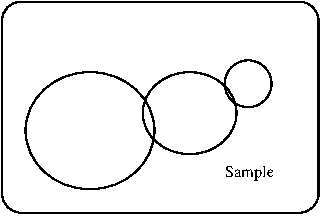
\includegraphics[width=5.8cm,keepaspectratio]{figure.pdf}\\
  \end{center}
  \caption{図の例}%
\label{fig1}
\end{figure}

キャプションは図の場合は下,表の場合は上に入れます.図や表を入れた場合,
必ず参照番号を使った文章を本文に入れます.
例: 図\ref{fig1} は図の,表\ref{table1}は表のサンプルである.

文献引用には,必ず\verb+\cite+を使用してください.例: 表\ref{table1}に,
文献\cite{labelName}で使用された計算機の仕様を示す.

\begin{table}[!htb]
 \begin{center}
   \caption{表の例}
  \begin{tabular}{|c|l|} \hline
  OS &  Linux 4.4.92(64bit) \\ \hline
  CPU & Intel Core i7-7700@3.60GHz\\ \hline
 メモリ & 62.8GByte\\ \hline
  \end{tabular}
 \label{table1}
 \end{center}
\end{table}


\section{結 論}
毎年同様の手引書が配布されていますが,その
中に書かれている注意に従わない予稿を多数目にします.必ずこの手引きの指
示に従って作成し,指導教員の許可を得てから提出してください.
%□□□□□□□□□□□□□□□□□□□□□□□□□□□□□□□□
%□□□□□□□□□□


%本来は\cite{kinosita}等として、本文中で引用された文献のみリストに
%掲載されます。\nociteは本文で引用されていない文献をリストに加える
%命令なので、実際に予稿を作成する際には使用してはいけません。
\nocite{kinosita}
\nocite{suetake}
\nocite{labelName}


\makeatletter
\def\@biblabel#1{#1)}
\makeatother

%下記は半自動で文献リストを生成する方法です。
%できれば、全自動で文献リストを生成するbibTeXを
%使用してください。

%bibTeXを使う場合は、ここから
\begin{thebibliography}{1}

\bibitem{kinosita}
木下是雄:理科系の作文技術, 中公新書 624 (1981).

\bibitem{suetake}
末武国弘:科学論文をどう書くか, 講談社ブルーバックス (1981).

\bibitem{labelName}
第1著者, 第2著者:論文名(論文の場合のかき方), 論文誌名, 巻番号, 号番号, pp.
  31--38 (2018).
\end{thebibliography}
%ここまでをコメントアウトして以下の\bibliographyの行のコメントアウトを解除し、
%pbibtexコマンドを実行してください。

%\bibliography{reference}

\bibliographystyle{tipsj}   



\end{document}